%

%%%%%%%%%%%%%%%%%%%%%%%%%%%%%%%%%%%%%%%%%%%%%%%%%%%%%%%%%%%%%%%%%%%%%%%%
\chapter{Plugin Implementation}
\label{chap:PluginImplementation}

\blindtext[1]

%%%%%%%%%%%%%%%%%%%%%%%%%%%%%%%%%%%%%%%%%%%%%%%%%%%%%%%%%%%%%%%%%%%%%%%%
\section{Goals}
\label{sec:goals}

\blindtext[2]

%%%%%%%%%%%%%%%%%%%%%%%%%%%%%%%%%%%%%%%%%%%%%%%%%%%%%%%%%%%%%%%%%%%%%%%%
\section{Implementation details}
\label{sec:implementationDetails}

\blindtext[1]

%%%%%%%%%%%%%%%%%%%%%%%%%%%%%%%%%%%%%%%%%%%%%%%%%%%%%%%%%%%%%%%%%%%%%%%%

\subsection{Key Features}
\label{sec:keyFeatures}

\blindtext[2]

\subsection{User Interface}
\label{sec:userInterface}

\blindtext[8]

\subsection{Architecture}
\label{sec:Architecture}

\blindtext[8]

%%%%%%%%%%%%%%%%%%%%%%%%%%%%%%%%%%%%%%%%%%%%%%%%%%%%%%%%%%%%%%%%%%%%%%%%

\section{Encountered Problems}
\label{sec:encounteredProblems}

In this section, I will discuss the main problems I encountered during implementation. To briefly summarize, they mainly consisted of how to create a simple, intuitive user interface and how the system behind the interface should be designed to have the best or at least a reasonable performance. \\ In the other visualizations, I noticed that I was quite overwhelmed by the amount of buttons which were visible, even though not always enabled. So I wanted to keep my user interface as simple as possible while not restricting the user in his ability to navigate through the visualization. \\ Regarding the performance, the author of the AES visualization has mentioned in his thesis that to create a fluent user experience where he can navigate back and forth between all steps, the intermediate values need to be calculated beforehand and saved since we don't want to stop at each step to calculate the next value or recalculate everything from the start if the user wants to go backwards. I came to the same conclusion. But as I will describe on the next pages, this was not all that was needed to ensure such an experience.\\
I hope that the description of these problems and the solutions I have found may help future students in writing their own plugins.

\subsection{Performance}

The peformance of the plugin was essentially coupled to how the navigation system was designed. Other things like the aforementioned calculation of the intermediate values for the visualization were compared to the navigation system design unsignificant because they are created by the ChaCha cipher anyway and must just be saved somewhere to not lose them. This means that storing them was only a necessary but not sufficient condition for a overall good performance. I realized this early in development when I had my first page with many page actions on it and wanted to skip ahead a lot of actions. While implementing this feature which would enable the user to skip from any action to any other action, I realized that when skipping more than 100 actions, it already took about 750ms during which the UI was unresponsive. As can be seen in \ref{navsystem.linear.stats}, this time increased linearly so it was quite clear that I needed to do something about this, especially because the page with the most actions had over 3000 single actions.

\par

The root cause of the problem was the navigation system design which I called in hindsight \textbf{\textit{linear navigation system}}. It consisted of defining actions which build upon each other. This means that if we are at action 0 (initial state of the page) and want to go to action 5, we need to execute all the code inside the action definitions between 0 and 5 to arrive at the page state as it should be at action 5. This is resembled in Figure \ref{navsystem.linear.overview}.

\begin{figure}
\caption{Navigation paths between actions in the linear navigation system}
\label{navsystem.linear.overview}
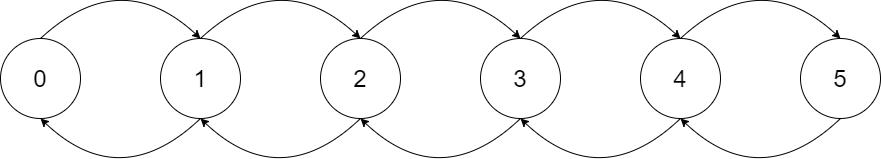
\includegraphics[width=\textwidth]{figures/navigationsystem-linear-overview.png}
\end{figure}

I came up with this design to have a smooth implementation experience where I only have to write the actual page state changes between two actions instead of duplicating a lot of code since the page state changes which were applied during a previous page were most of the times still visible when moving to the next action. This complements how the user experiences the visualization because the actions are numbered in a sequence and thus are inherently linear. Because of this, it made a lot of sense to me to reflect this in the system architecture.

\par

Since this "design flaw" was not the leading cause of the performance problem (going through a for-loop of size 3000 does not directly lead to performance issues), I want to briefly explain how the actual action implementation looked like.\\
As can be seen in Figure \ref{navsystem.linear.detail}, during the transition between two page states, the state of the page elements which will change is saved such that we can undo the changes if the user decides to navigate back. This enabled me to skip writing action definitions for backwards navigation, since I could just write a function which retrieves the state corresponding to the transition and then applies it. This function would then work for all backwards navigation without further intervention which was very convenient during development.
The problem with that architecture was that the state saving and the execution logic inside the action definitions were changing a lot of page elements directly by accessing them via their name that I gave them in the XAML code. That this was against best practices in writing WPF applications I only noticed later on, when I read more about them. This issue combined with the restricted, linear pathing between actions resulted in that huge performance loss that was described in Figure \ref{navsystem.linear.stats}.

\par

After identifying the two underlying issues, I implemented what I called a \textbf{\textit{linear navigation system with caches}}. As the name suggests, I implemented cache entries to be able to navigate in constant time between an action and an action for which I created a cache. To not only increase peformance during these transitions but between all transitions, we check before each transition, if first moving to a cached entry would decrease the amount of hops needed to go to our destination.\\
The cache entries consisted of instructions to restore the complete state of a page at the action index for which this cache entry was for. They contained instructions for the complete state instead of only the difference between two actions because now, moving to that cache must initialize the page from any other action. But this was no problem since the cache entries were written into the code and not generated during run time, therefore, this had only a performance impact during compile time, not during run time. Figure \ref{navsystem.cache.overview} demonstrates that the navigation system now needs less hops between any two given actions. This increased performance significantly as can be seen in \ref{navsystem.cache.stats}. \par

\begin{figure}
\caption{Navigation paths between actions in the linear navigation system with caches. The colorized state has a corresponding cache entry.}
\label{navsystem.cache.overview}
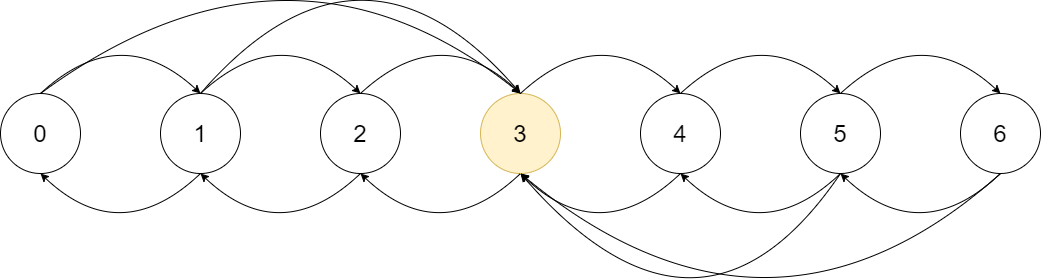
\includegraphics[width=\textwidth]{figures/navigationsystem-cache-overview-2.png}
\end{figure}

One of the major drawbacks for this enhanced design was that the automatic action undoing was no longer possible. Since we can not guarantee that the state between two actions has been saved, we cannot use our undo function. The reason is that any transition between two actions may have been skipped because first moving to a cached entry needed less hops. Therefore, I needed to write the code for backwards navigation to support caching.

\par


